\section{Design}
\label{sec:design}
We describe the evolution of the design of \system{} starting with an initial strawman approach.  We then 
alter the design as we address each of the design goals discussed in the previous section (and in Table \ref{tab:design_goals}), which brings us 
to a complete design.

\subsection{Strawman: Hiding Information From CDN}
\label{sec:obfuscate_content}
To prevent an inside attacker or overreaching government from learning information, the CDN 
must not have the knowledge of what content it is caching.  Therefore, the content {\it and} the 
associated URL must be obfuscated before they enter the CDN.  

\paragraph{Encrypt Content.}  The content can be obfuscated by encrypting it with a key that is not 
known to the CDN.  Because this must be done prior to any caching, the content publisher 
has to generate some key $k$ to encrypt the content with.  Then this encrypted (and subsequently 
obfuscated) content is then sent to the CDN\footnote{Most CDNs
allow the publisher to decide on a push or pull model, but this makes no difference in our 
system design.} and stored in its caches.  
Additionally, if the domain supports HTTPS requests, then the content publisher must also encrypt the 
associated certificate with the same key $k$.  This content and certificate must be decrypted after 
it leaves the CDN; the client could decrypt the certificate and check its validity.  If valid, then 
the client uses $k$ to decrypt the content.  

\paragraph{Obfuscate URL.} Encrypting the content alone does not hide much from the CDN; the content 
identifier, or URL, must also be obfuscated, otherwise the CDN can still reveal information about 
which clients accessed which URLs (which is indicative of the content).  In obfuscating the 
URL, the result should be a fixed, and relatively small size; these requirements are to preserve 
storage space and to prevent the adversary from guessing the URL based on the length of the obfuscated 
URL.  Hashing the URL provides these 
properties, and hides the actual URL from the CDN. With obfuscated content and 
URLs, the CDN does not know what content a given client is accessing.

\paragraph{Client Anonymization.}  The CDN may not know the content that a client is accessing, but it 
still knows information about the clients that are accessing any content at the CDN.  It knows 
where the clients are located and how many times they are accessing any content.  To address this, 
a client can simply use an anonymizing proxy or VPN when accessing content.  This hides a certain 
amount of information about the client, including the client's location and a direct link of 
client to content request.

This strawman approach obfuscates content from the viewpoint of the CDN, which also allows the CDN 
to claim plausible deniability when served with a subpoena.  Despite only cachine encrypted and obfuscated 
content and identifiers, the CDN still has knowledge of which clients are requesting any content and how often 
they are requesting content.  Unfortunately, this approach raises 
many questions: are anonymizing proxies/VPNs trustworthy?, should clients be trusted to know $k$?, 
can any jurisdiction still subpoena the CDN for information (presumably the CDN has locations in many 
countries and clients in many countries)?

%, do malicious clients have more power as the CDN's attack 
%detection and prevention capabilities are severely limited?

\subsection{Moving Jurisdictions}
As it is still unclear which jurisdiction is legally allowed to subpoena information from the CDN (such as which 
clients are accessing any content distributed by the CDN), this 
system should complement the legal framework; it should make clear which jurisdictions are allowed 
which information, and also prevent an overreaching government from demanding data.  This 
can be addressed by introducing a closed system of proxies, where a client uses a single proxy when requesting 
content --- not only does this proxy provide a level of client anonymity, but also decides which jurisdiction 
the data falls under.  

\paragraph{Proxy in Client's Jurisdiction.} By replacing the use of an anonymizing proxy or VPN with the use 
of a proxy---one that is part of \system{} and supplied to clients based on their location---, the system can specify which juridiction each client falls under.  For example, 
each country could have a set of proxies, where all clients in each country use one of the proxies that 
is located in their country.  This should allow the client's jurisdiction to serve a subpoena for information 
passing through the specific proxy that a client uses in the client's jurisdiction in 
necessary criminal investigations, but prevents any other jurisdiction from demanding data on the same 
client because the subpoena must be served for a specific proxy.  While it appears that the source of 
trust is simply shifted from the CDN to the proxy, the use of this proxy is essential in 
the system design for a number of reasons.  First, the use of proxies distributes trust; instead of a 
central entity, the CDN, having access to all information, it is now a set of proxies that each have 
access to some subset of information.  Each proxy only knows information about a much smaller set of clients.  
Additionally, the proxy does not cache content or keep state, whereas the CDN does both of these.  Apart 
from addressing jurisdictional issues, proxies also improve usability; instead of each client having knowledge 
of each $k$ for each domain, each proxy could have knowledge of each $k$.  This means that clients would 
not have to keep track of secret knowledge, and overall, the number of entities that know this secret key 
is much smaller (as the number of proxies is significantly smaller than the number of clients).  Lastly, 
the proxy can perform attack detection and prevention before the attack even reaches the CDN; more optimizations 
made possible by the use of proxies are discussed in Section \ref{sec:optimizations}.

\paragraph{Decouple Content Distribution from Decision of Trust.} Using proxies also separates the issues of 
trust and content distribution.  A client no longer needs to trust the CDN, which all other clients would 
need to trust as well.  Now the client can simply trust the proxy, which interacts with the CDN; this proxy 
is a completely separate entity from the CDN.  Therefore this design allows a client to decouple these 
issues, where she can trust only a proxy, not the CDN, but still access cached content at the CDN.

\subsection{Reducing Attack Surface}
The design has evolved into a system where: 1) the CDN does not know the content, the content identifier, 
or which clients are accessing any content, 2) the client's data is only subject to subpoenas in her jurisdiction 
(or the jurisdiction of the proxy), 3) trust has been distributed, as opposed to centralized.  There are still 
some remaining security vulnerabilities that must be addressed.  First, the shared key $k$ for each content 
publisher is shared among all the proxies; therefore, if one proxy is compromised, then the key must be replaced 
on all proxies.  Second, simply hashing the URL allows an attacker who simply 
wishes to guess whether the obfuscated URL is a specified plaintext URL or not.  By increasing the number of shared 
keys $k$ and introducing shared secrets to URL obfuscation, the design reduces the probability of attacks.

\paragraph{Increasing the Number of Keys.} If a single shared key $k$ associated with a single content publisher gets 
compromised, then all proxies have a compromised $k$ for that content publisher.  By increasing the number of shared 
keys that a content publisher uses to encrypt her content, this decreases the fraction of proxies that use a 
compromised key given that one of the keys is compromised.  Instead of a content publisher encrypting content with a 
single key, she will encrypt a copy of the content with different keys.  If there are $n$ shared keys, then there 
will be $n$ copies of the content, where each copy is encrypted with a different shared key.  To maximize security, each proxy should share a
different $k$ with the content publisher; unfortunately, this defeats the purpose of CDNs caching content.  If each 
proxy is requesting a unique copy of the content, then cache hit rates decrease and performance becomes worse.  To make 
a tradeoff between security and performance, there should be $n$ keys where $1 < n < |proxies|$, such that subsets of 
proxies share the same shared key $k$ with the content publisher.  If one of these shared keys is leaked (or otherwise learned), only that 
subset of proxies that use that shared key must get a new key.  

\paragraph{Adding Secrecy to URL Obfuscation.} According to the strawman approach, the URL is obfuscated via hashing.  Unfortunately, 
an attacker could guess what the content identifier is by hashing his guesses and comparing with the hashes stored in the 
CDNs caches.  To mitigate this vulnerability, the content publisher should incorporate the use of the shared key $k$ in the 
hash of the URL by using an HMAC.  This provides the property of fixed length identifiers, which does not reveal information about 
the plaintext identifiers, while obfuscating and preventing 
against guessing attacks.  

The resulting system is the basis of \system{}, and the high-level view of the system is shown in Figure \ref{fig:ocd_overview}, 
which can be compared to what CDNs look like today (Figure \ref{fig:basic_cdn}).  The next section describes \system{} in more 
detail and outlines the specific steps for publishing and retrieving content.

\begin{figure}[t]
\centering
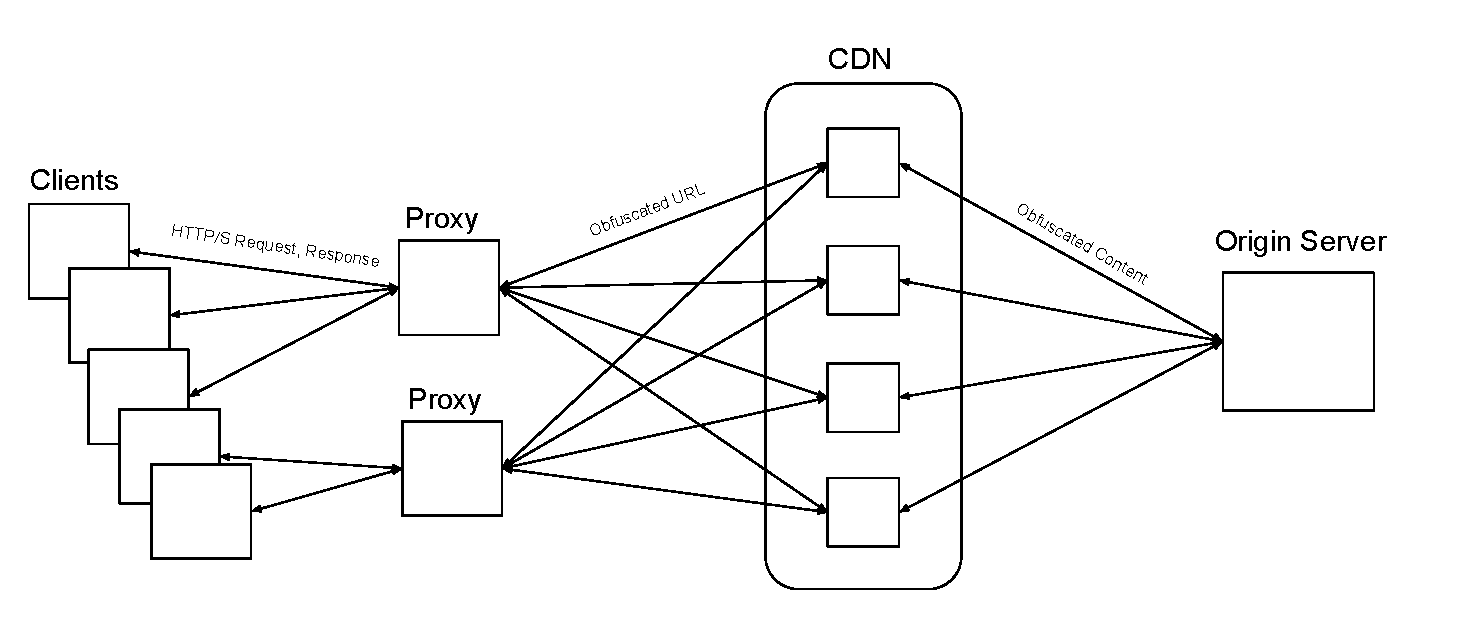
\includegraphics[width=.5\textwidth]{full_ocd_system}
\caption{The relationships between clients, the CDN, proxies, and content publishers in 
\system{}.}
\label{fig:ocd_overview}
\end{figure}
